\documentclass[
  bibliography=totoc,     % Literatur im Inhaltsverzeichnis
  captions=tableheading,  % Tabellenüberschriften
  titlepage=firstiscover, % Titelseite ist Deckblatt
]{scrartcl}

% Paket float verbessern
\usepackage{scrhack}

% Warnung, falls nochmal kompiliert werden muss
\usepackage[aux]{rerunfilecheck}

% unverzichtbare Mathe-Befehle
\usepackage{amsmath}
% viele Mathe-Symbole
\usepackage{amssymb}
% Erweiterungen für amsmath
\usepackage{mathtools}

% Fonteinstellungen
\usepackage{fontspec}
% Latin Modern Fonts werden automatisch geladen
% Alternativ zum Beispiel:
%\setromanfont{Libertinus Serif}
%\setsansfont{Libertinus Sans}
%\setmonofont{Libertinus Mono}

% Wenn man andere Schriftarten gesetzt hat,
% sollte man das Seiten-Layout neu berechnen lassen
\recalctypearea{}

% deutsche Spracheinstellungen
\usepackage[english]{babel}


\usepackage[
  math-style=ISO,    % ┐
  bold-style=ISO,    % │
  sans-style=italic, % │ ISO-Standard folgen
  nabla=upright,     % │
  partial=upright,   % │
  mathrm=sym,        % ┘
  warnings-off={           % ┐
    mathtools-colon,       % │ unnötige Warnungen ausschalten
    mathtools-overbracket, % │
  },                       % ┘
]{unicode-math}

% traditionelle Fonts für Mathematik
\setmathfont{Latin Modern Math}
% Alternativ zum Beispiel:
%\setmathfont{Libertinus Math}

\setmathfont{XITS Math}[range={scr, bfscr}]
\setmathfont{XITS Math}[range={cal, bfcal}, StylisticSet=1]

% Zahlen und Einheiten
\usepackage[
  locale=DE,                   % deutsche Einstellungen
  separate-uncertainty=true,   % immer Unsicherheit mit \pm
  per-mode=symbol-or-fraction, % / in inline math, fraction in display math
]{siunitx}

% chemische Formeln
\usepackage[
  version=4,
  math-greek=default, % ┐ mit unicode-math zusammenarbeiten
  text-greek=default, % ┘
]{mhchem}

% richtige Anführungszeichen
\usepackage[autostyle]{csquotes}

% schöne Brüche im Text
\usepackage{xfrac}

% Standardplatzierung für Floats einstellen
\usepackage{float}
\floatplacement{figure}{htbp}
\floatplacement{table}{htbp}

% Floats innerhalb einer Section halten
\usepackage[
  section, % Floats innerhalb der Section halten
  below,   % unterhalb der Section aber auf der selben Seite ist ok
]{placeins}

% Seite drehen für breite Tabellen: landscape Umgebung
\usepackage{pdflscape}

% Captions schöner machen.
\usepackage[
  labelfont=bf,        % Tabelle x: Abbildung y: ist jetzt fett
  font=small,          % Schrift etwas kleiner als Dokument
  width=0.9\textwidth, % maximale Breite einer Caption schmaler
]{caption}
% subfigure, subtable, subref
\usepackage{subcaption}

% Grafiken können eingebunden werden
\usepackage{graphicx}

% schöne Tabellen
\usepackage{tabularray}
\UseTblrLibrary{booktabs, siunitx}
\usepackage{longtable}

\DefTblrTemplate{contfoot-text}{normal}{Weiter auf der nächsten Seite}
\SetTblrTemplate{contfoot-text}{normal}
\DefTblrTemplate{conthead-text}{normal}{(Fortsetzung)}
\SetTblrTemplate{conthead-text}{normal}

% Verbesserungen am Schriftbild
\usepackage{microtype}

% Literaturverzeichnis
\usepackage[
  backend=biber,
]{biblatex}
% Quellendatenbank
\addbibresource{lit.bib}
\addbibresource{programme.bib}

% Hyperlinks im Dokument
\usepackage[
  german,
  unicode,        % Unicode in PDF-Attributen erlauben
  pdfusetitle,    % Titel, Autoren und Datum als PDF-Attribute
  pdfcreator={},  % ┐ PDF-Attribute säubern
  pdfproducer={}, % ┘
]{hyperref}
% erweiterte Bookmarks im PDF
\usepackage{bookmark}

% Trennung von Wörtern mit Strichen
\usepackage[shortcuts]{extdash}

% Schriftfarbe ändern
\usepackage{xcolor}

\begin{document}

\section*{\Huge \textbf{Regularization Submission}}

\subsection*{Problem 1}

Comparing a small/normal neural network, as seen in \autoref{fig:Fig01}, to a large and deep neural network in \autoref{fig:Fig02}, 
they are almost identical to each other.
The only real difference is a small overfitting that can be observed in the large NN with increasing epochs.
\begin{figure}[H]
  \centering
  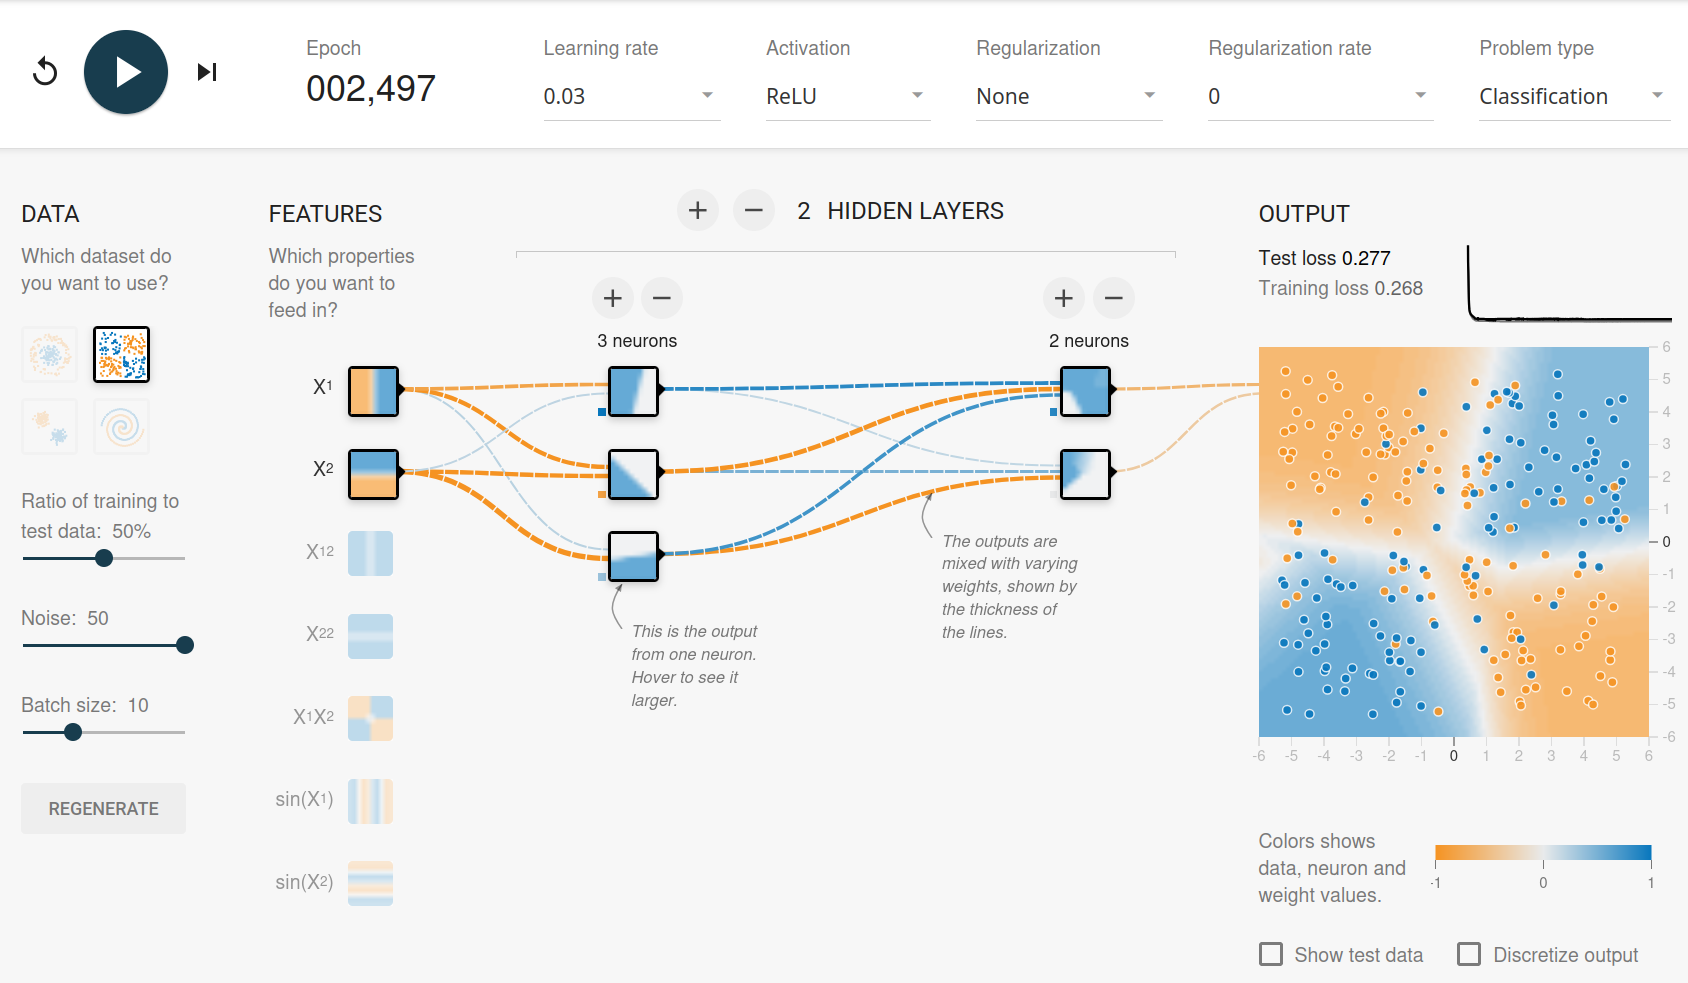
\includegraphics[width=0.85\textwidth]{Small_NN.png}
  \caption{Small Neural Network with two layers and 5 neurons together.}
  \label{fig:Fig01}
\end{figure}

\begin{figure}[H]
  \centering
  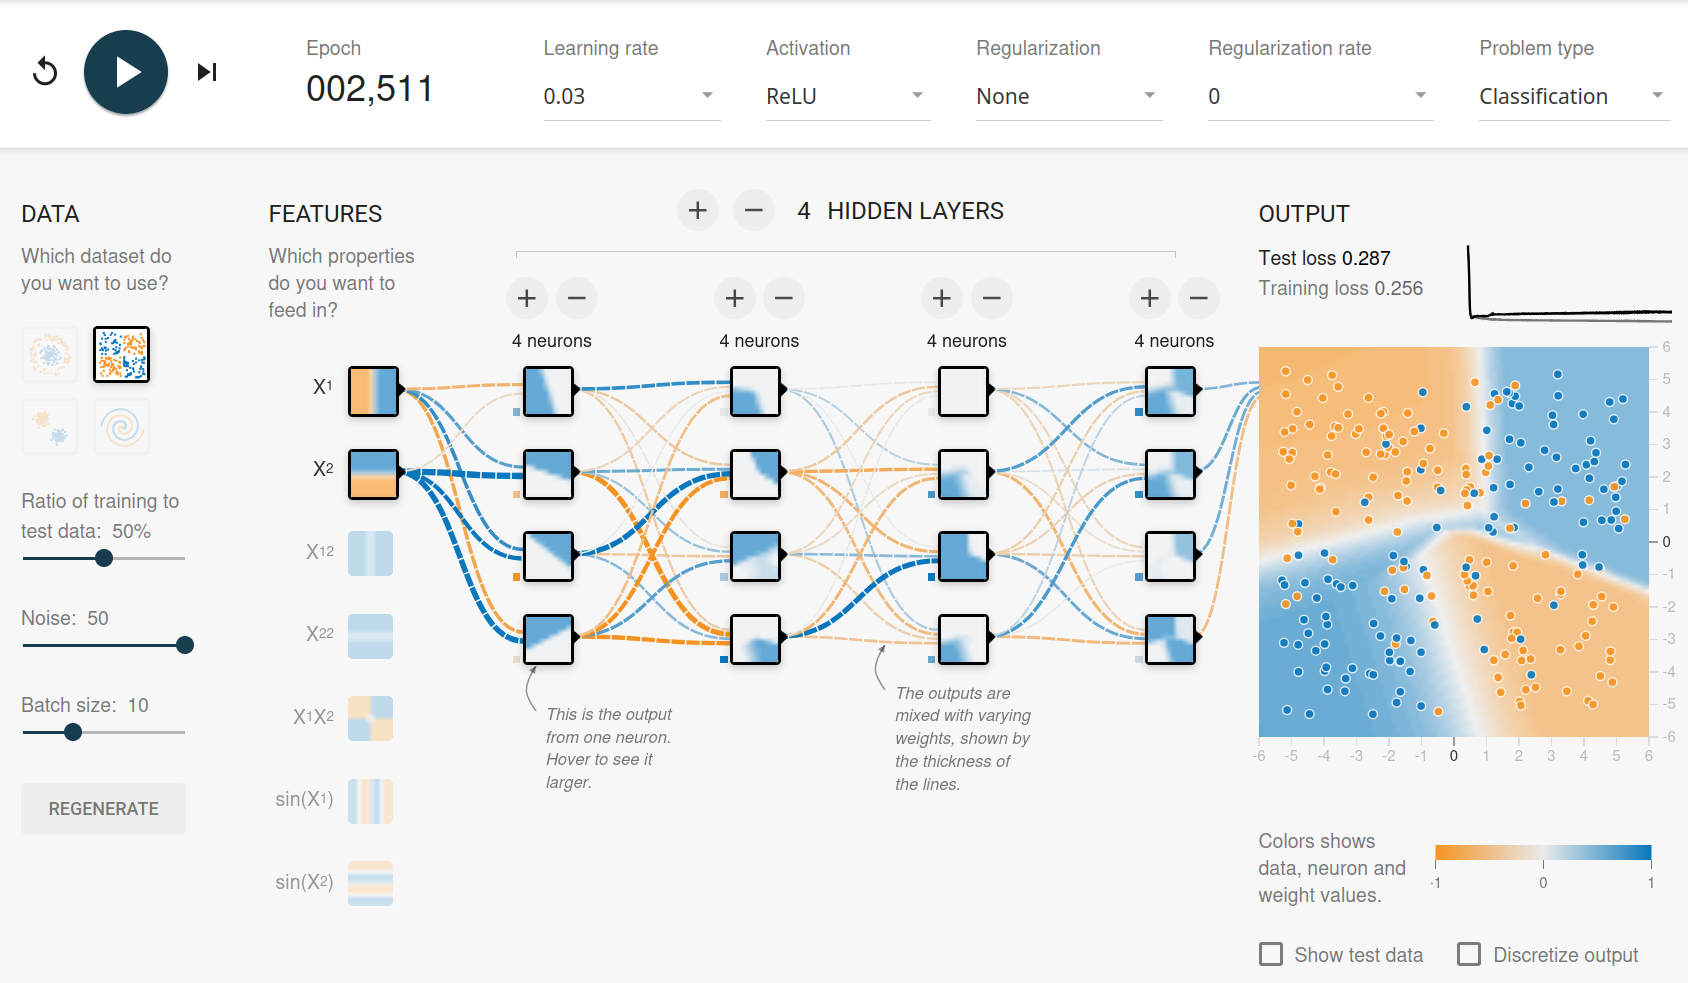
\includegraphics[width=0.85\textwidth]{Big_NN.png}
  \caption{Large Neural Network with 4 layers and 4 neurons each.}
  \label{fig:Fig02}
\end{figure}

\subsection*{Problem 2}

When adding the L2-Regularization, the overfitting of the training doesn't occur anymore,
as seen in \autoref{fig:Fig03}.

\begin{figure}[H]
  \centering
  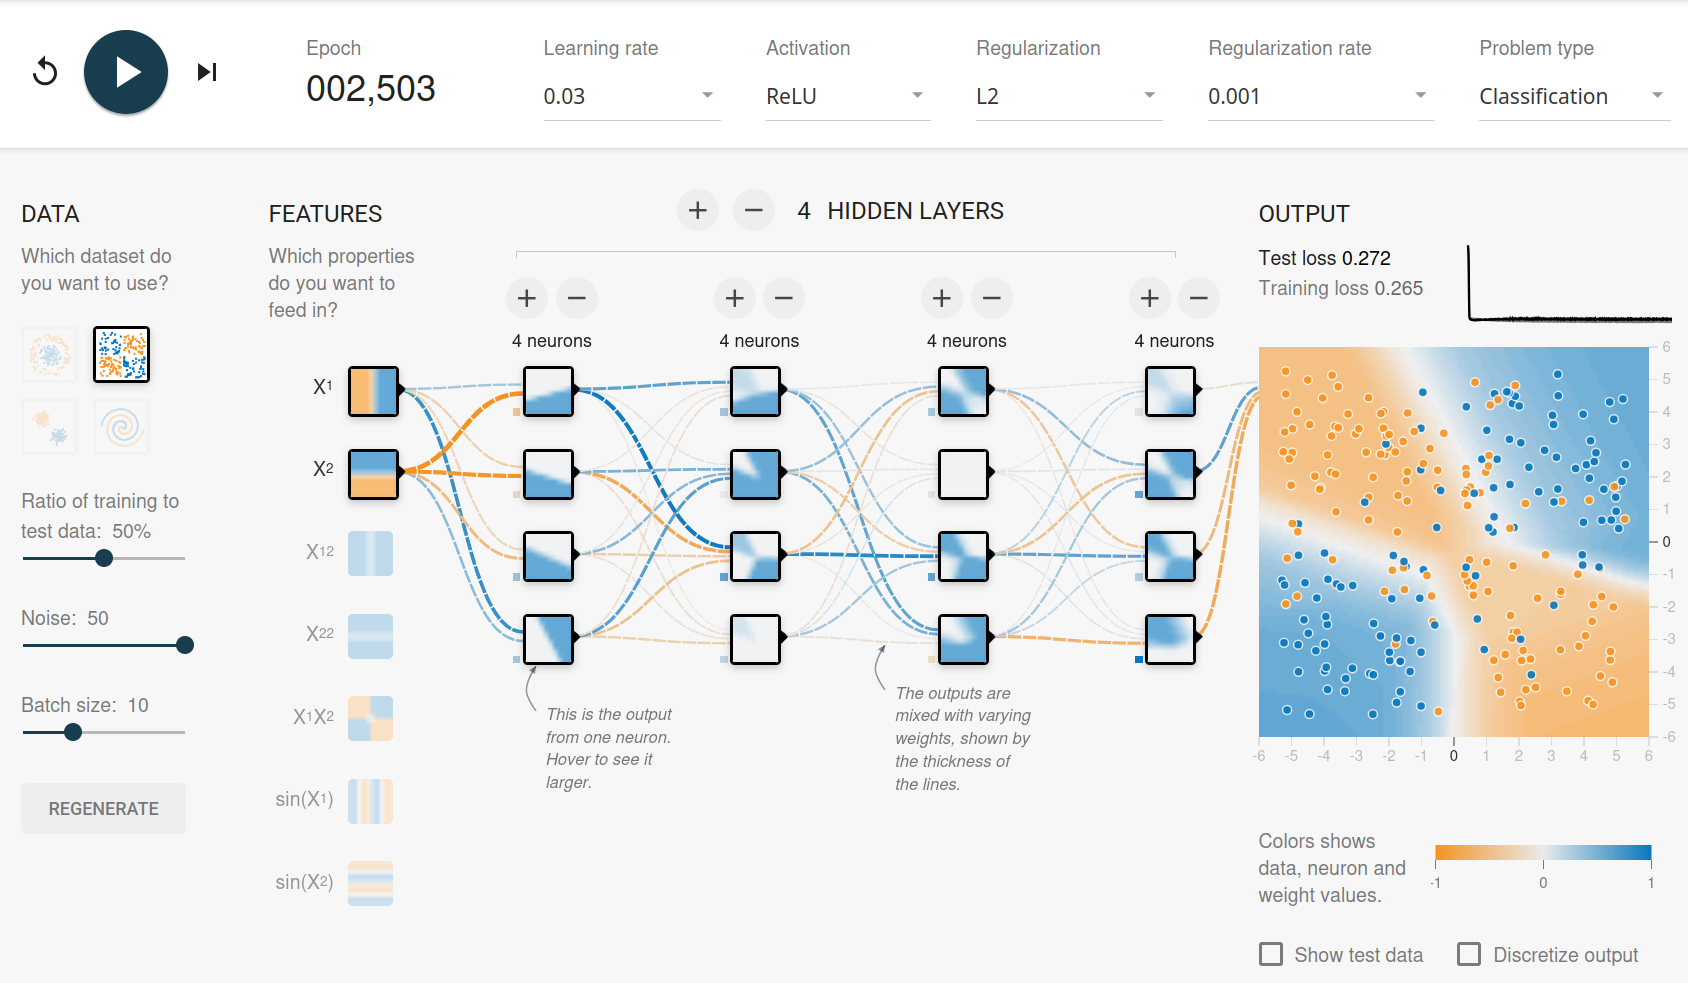
\includegraphics[width=0.85\textwidth]{Small_L2.png}
  \caption{Overfitted NN with a small L2-Regularization of \qty{0.001}{}.}
  \label{fig:Fig03}
\end{figure}

This only works for small regularization rates. If the rates are too high, as seen in \autoref{fig:Fig04} and \autoref{fig:Fig05},
the network is flattened out and the single points can't be sorted into orange or blue as efficient as before. 
(Since their weights would be too high.)
With extreme high rates (\autoref{fig:Fig05}), the NN becomes useless, as the loss function won't decrease anymore and almost no point is classified at all.

\begin{figure}[H]
  \centering
  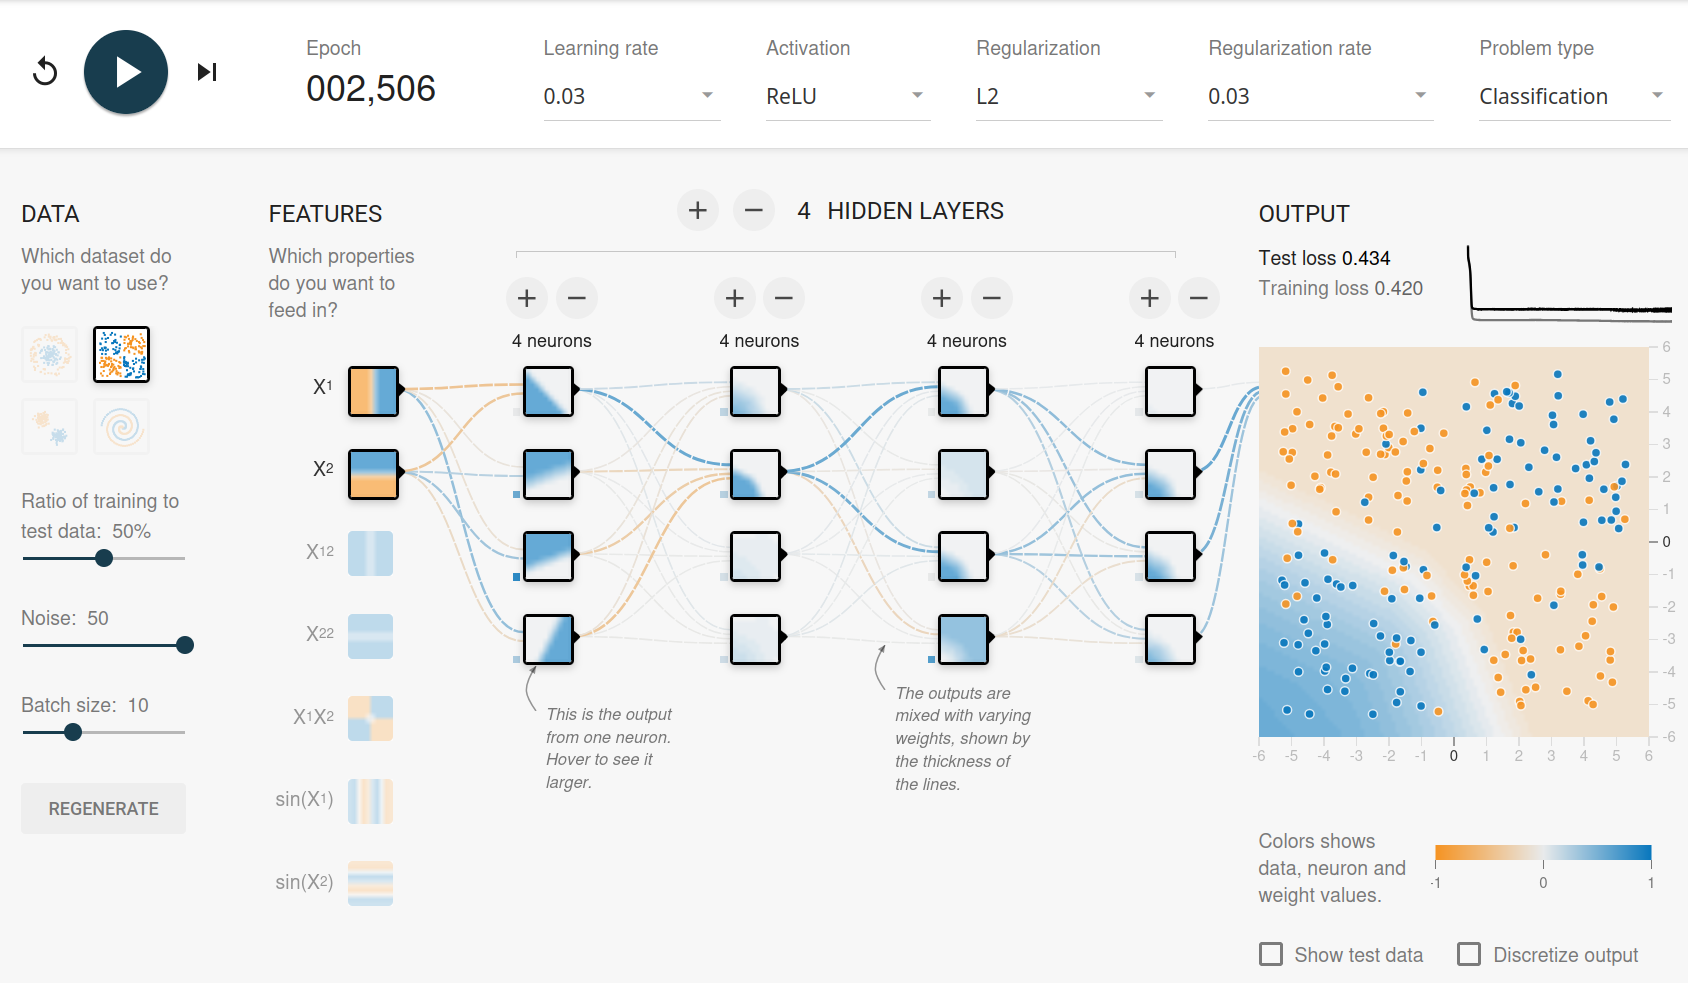
\includegraphics[width=0.85\textwidth]{Middle_L2.png}
  \caption{Overfitted NN with a medium L2-Regularization of \qty{0.03}{}.}
  \label{fig:Fig04}
\end{figure}

\begin{figure}[H]
  \centering
  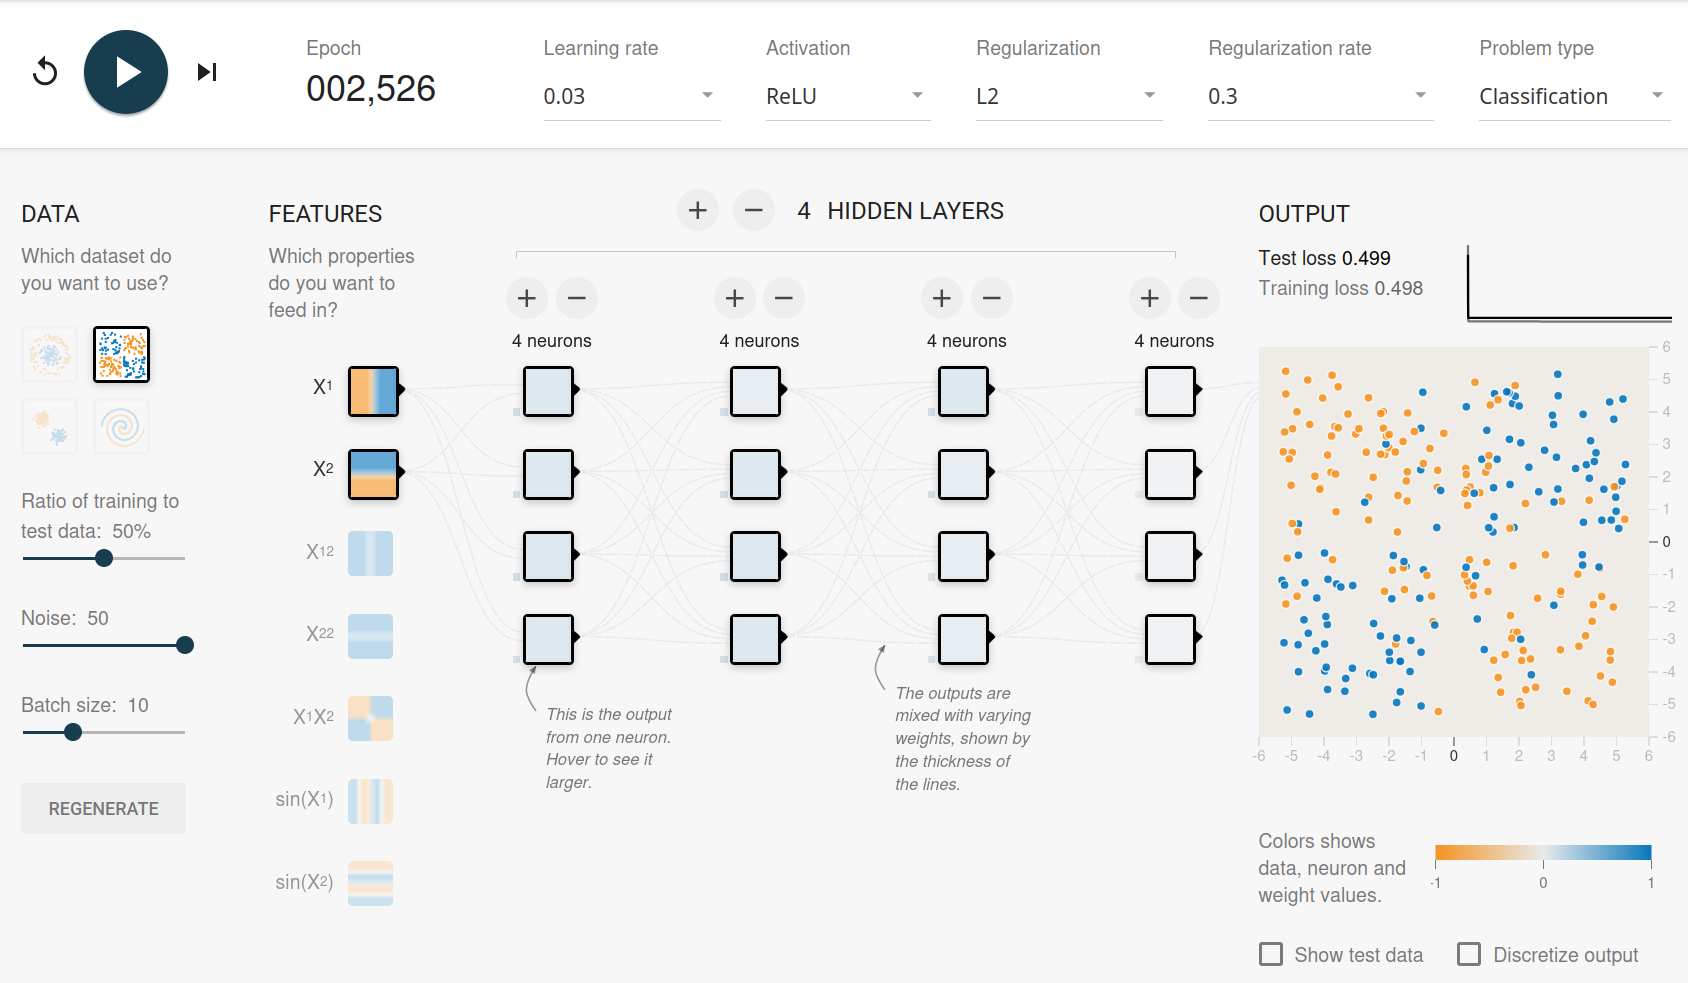
\includegraphics[width=0.85\textwidth]{Big_L2.png}
  \caption{Overfitted NN with a large L2-Regularization of \qty{0.3}{}.}
  \label{fig:Fig05}
\end{figure}

\newpage
\subsection*{Problem 3}

Comparing \autoref{fig:Fig03} and \autoref{fig:Fig06}, the biggest difference between the L1- and L2-Regularization is visible in their weights.
While the L2-Regularization only reduces the weights, the L1-Regularization sets some of them to zero, effectively shutting down some of the neurons.

\begin{figure}[H]
  \centering
  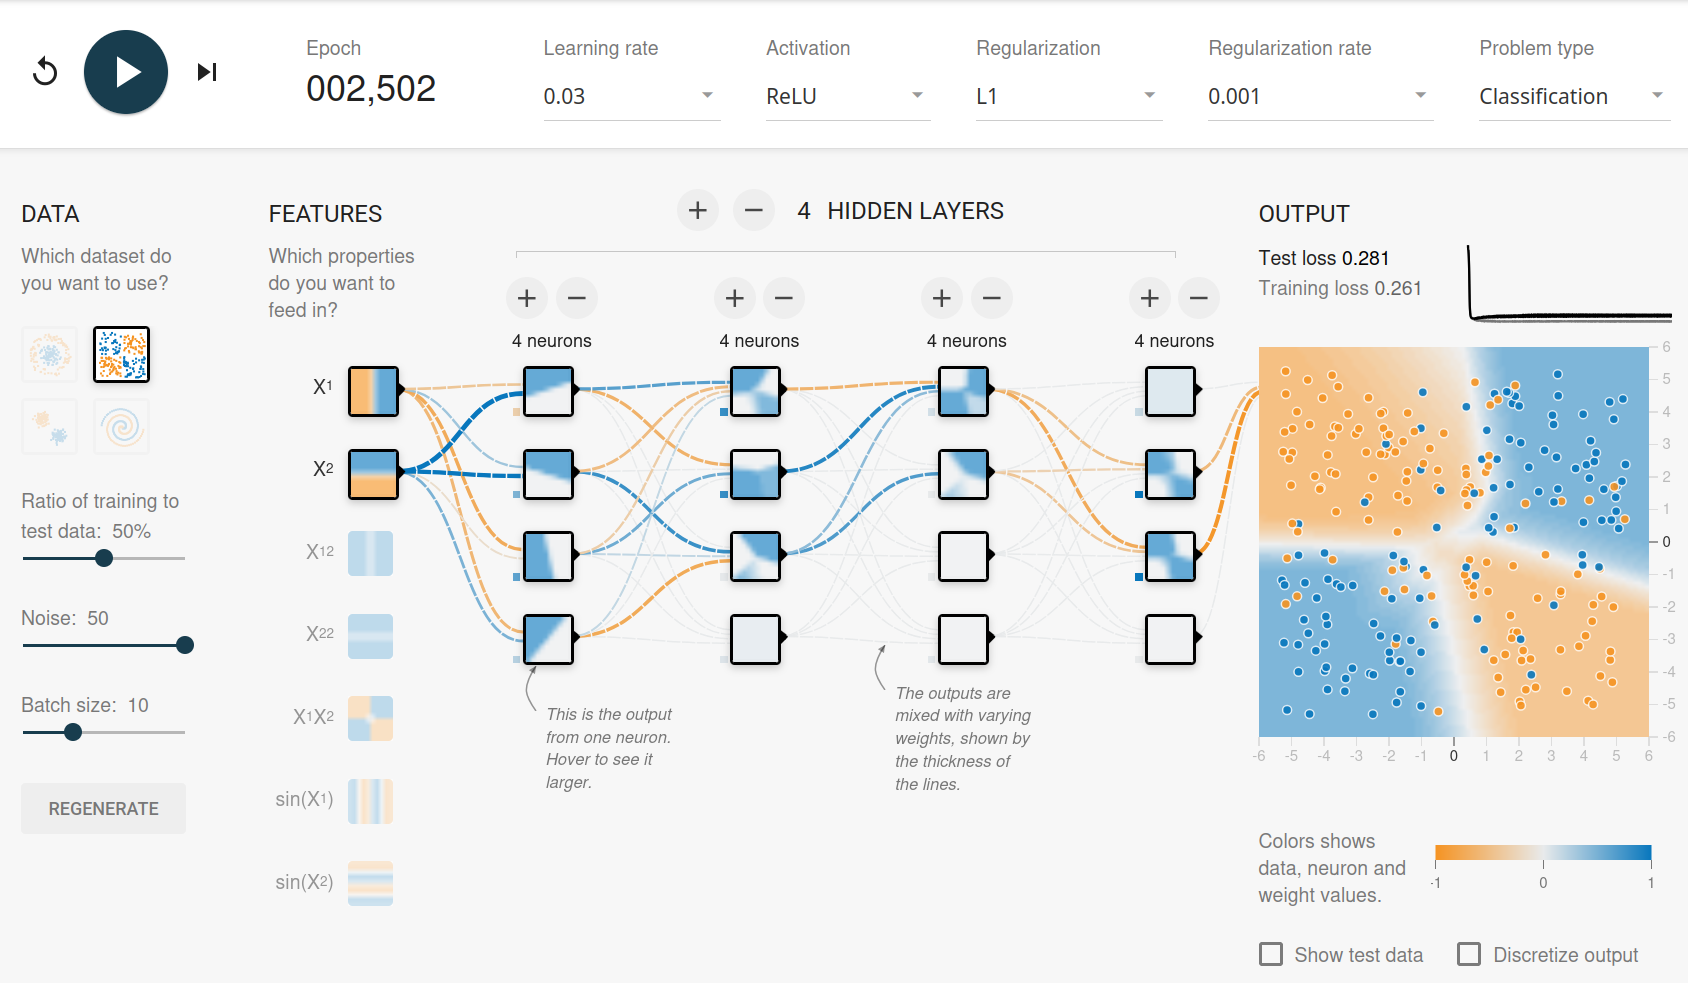
\includegraphics[width=0.85\textwidth]{Small_L1.png}
  \caption{Overfitted NN with a small L1-Regularization of \qty{0.001}{}.}
  \label{fig:Fig06}
\end{figure}

This can result in a NN that relies on less features, making the NN more selective.

\end{document}
